\documentclass[12pt, a4paper]{article}
\usepackage[utf8]{inputenc}
\usepackage{geometry}
\geometry{a4paper, margin=1.2in}
\usepackage{graphicx}
\usepackage{setspace}
\usepackage{hyperref}
\usepackage{fancyhdr}
\usepackage{booktabs}
\usepackage{float}
\usepackage{tikz}
\usepackage{tabularx}
\usetikzlibrary{shapes.geometric, arrows.meta, positioning, calc}

\doublespacing

\begin{document}

\begin{titlepage}
    \centering
    \vspace*{2cm}
    
    \Huge
    \textbf{Software Design Document (SDD)}
    
    \vspace{0.5cm}
    \LARGE
    Project: Nucleus
    
    \vspace{1.5cm}
    
    \textbf{Continuous Behavioral Authentication and CI/CD Orchestration System}
    
    \vspace{2cm}
    
    \Large
    \textbf{Prepared by:} \\
    Shlok Burmi \\
    Yuvraj \\
    Sujal Kishore \\
    
    \vfill
    
    \Large
    \textbf{Date:} \today \\
    
\end{titlepage}

\tableofcontents
\newpage
\listoffigures
\newpage
\listoftables
\newpage

\section{Introduction}
\subsection{Purpose}
The purpose of this Software Design Document (SDD) is to detail the architectural and structural logic of the "Nucleus" project. It outlines the translation of system requirements as articulated in the SRS into software components, modules, interfaces, and data architectures. 

\subsection{Scope}
This SDD encompasses the full technology stack utilized in Nucleus: React frontend implementations, Node.js/Express backend APIs, MongoDB schemas, Jenkins CI/CD architectural pipelines, and Python-based LSTM machine learning inference segments.

\subsection{Overview of Document}
This document outlines system architecture in Section 3, followed by Data Layer configurations in Section 4, component module logic in Section 5, and the continuous deployment blueprint in Section 6.

\newpage
\section{System Overview}
The software executes a multi-tiered pattern comprising separated logic layers to maximize modularity. Standard OAuth paradigms handle entry, whereupon constant background tracking streams metadata to a machine learning array. A dedicated Continuous Integration server ensures testing boundaries and deploys updated microservices uniformly. 

\newpage
\section{System Architecture}

\subsection{Architectural Design}
The system follows a Microservices and Event-driven Architecture interconnected by API Gateways and WebSocket channels. Containerization is broadly adopted via Docker to maintain consistent application states.

\begin{figure}[H]
    \centering
    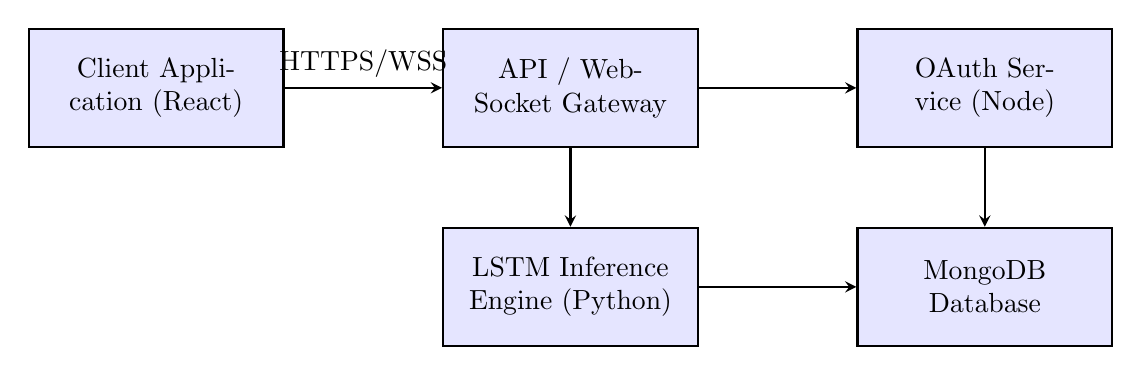
\begin{tikzpicture}[
        node distance=2cm,
        box/.style={rectangle, draw=black, thick, fill=blue!10, text width=3cm, align=center, minimum height=1.5cm},
        arrow/.style={thick, ->, >=stealth}
        ]
        
        \node[box] (client) {Client Application (React)};
        \node[box, right=of client] (gateway) {API / WebSocket Gateway};
        \node[box, right=of gateway] (auth) {OAuth Service (Node)};
        
        \node[box, below=1cm of gateway] (lstm) {LSTM Inference Engine (Python)};
        \node[box, below=1cm of auth] (db) {MongoDB Database};
        
        \draw[arrow] (client) -- node[anchor=south] {HTTPS/WSS} (gateway);
        \draw[arrow] (gateway) -- (auth);
        \draw[arrow] (gateway) -- (lstm);
        \draw[arrow] (auth) -- (db);
        \draw[arrow] (lstm) -- (db);
    \end{tikzpicture}
    \caption{High-Level Architectural Decomposition}
\end{figure}

\subsection{Design Rationale}
Decoupling the LSTM Inference loop from the standard REST API backend ensures heavy mathematical computations do not choke primary networking. Using Docker Compose creates reproducible local configurations simulating production clusters.

\newpage
\section{Data Design}

\subsection{Data Management}
Nucleus utilizes MongoDB for dynamic document-based persistence. It easily captures variable-length arrays needed for keystroke timings and coordinate streams.

\subsection{Entity-Relationship Dictionary}
\begin{table}[H]
\centering
\begin{tabularx}{\textwidth}{|X|X|X|X|}
\hline
\textbf{Entity} & \textbf{Field} & \textbf{Type} & \textbf{Description} \\
\hline
User & \texttt{\_id} & ObjectId & Primary Key \\
User & \texttt{oauth\_id} & String & External provider ref \\
User & \texttt{email} & String & Identifying address \\
Session & \texttt{session\_id} & String & JWT active token \\
Session & \texttt{is\_valid} & Boolean & Status flag \\
Behavioral & \texttt{x\_coords} & Array & Mouse X series \\
Behavioral & \texttt{y\_coords} & Array & Mouse Y series \\
Behavioral & \texttt{timestamp} & Array & Temporal markers \\
\hline
\end{tabularx}
\caption{Primary DB Entities and Types}
\end{table}

\newpage
\section{Component Design}

\subsection{Front-End Dashboard Components}
The UI reacts rapidly to inference outputs. An isolated `TrackingLayer` component acts as a high-order-component (HOC) wrapping secure spaces, triggering data acquisition vectors asynchronously.

\subsection{Back-End Routing Controllers}
Controllers map specific functionalities:
\begin{itemize}
    \item \texttt{/api/auth/*}: Handles standard entry protocols.
    \item \texttt{/api/stream/*}: Endpoint receiving chunked arrays of behavioral sets.
\end{itemize}

\subsection{Biometric API Pipeline}
LSTM sequences require normalized arrays padding up to 100 timesteps to output confidence logs. Data Cleaning utilities filter rapid sporadic noises before inference execution.

\newpage
\section{Continuous Delivery / Workflow Design}

\subsection{Jenkins Pipeline Operations}
The pipeline uses declarative syntaxes encoded in `Jenkinsfile`.

\begin{figure}[H]
    \centering
    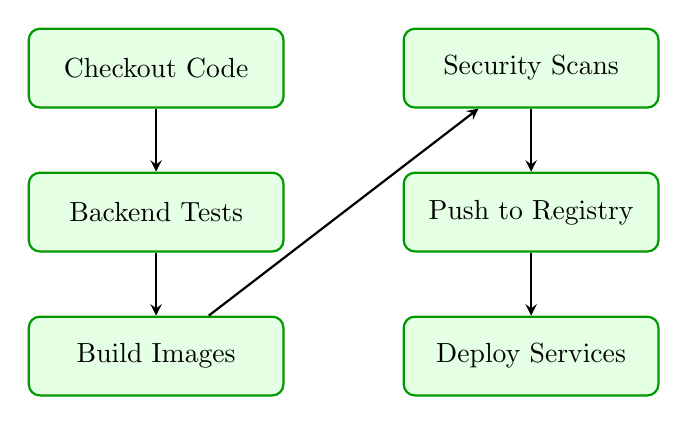
\begin{tikzpicture}[
        node distance=0.8cm and 1.5cm,
        box/.style={rectangle, draw=green!60!black, thick, fill=green!10, text width=3cm, align=center, minimum height=1cm, rounded corners},
        arrow/.style={thick, ->, >=stealth}
        ]
        
        \node[box] (checkout) {Checkout Code};
        \node[box, below=of checkout] (test) {Backend Tests};
        \node[box, below=of test] (docker) {Build Images};
        \node[box, right=of checkout] (scan) {Security Scans};
        \node[box, right=of test] (push) {Push to Registry};
        \node[box, right=of docker] (deploy) {Deploy Services};
        
        \draw[arrow] (checkout) -- (test);
        \draw[arrow] (test) -- (docker);
        \draw[arrow] (docker) -- (scan);
        \draw[arrow] (scan) -- (push);
        \draw[arrow] (push) -- (deploy);
    \end{tikzpicture}
    \caption{Declarative Jenkins Pipeline Flowchart}
\end{figure}

The pipeline executes robust tasks. \textbf{Checkout Code} pulls the latest main branch. \textbf{Backend Tests} verifies modules dynamically (Node interactions). \textbf{Build Docker Images} compiles frontend, backend, and inference components. \textbf{Security Scans} ensure zero vulnerabilities. \textbf{Push} stores configurations. \textbf{Deploy} instantiates orchestrated networks via Docker-compose logic natively.

\newpage
\section{Project Analytics Integration}

The Nucleus project tracked rigorous analytics over development sprints.

\subsection{GitHub Repository Analytics}
\begin{figure}[H]
    \centering
    \includegraphics[width=0.9\textwidth]{github_commits.png} % User MUST upload github_commits.png
    \caption{System Implementation Over Time - Commit Visualization}
\end{figure}
Deployment histories confirm the progressive enhancement pattern. Spikes correspond directly with resolution of critical Docker networking blocks and deployment validation.

\begin{figure}[H]
    \centering
    \includegraphics[width=0.9\textwidth]{github_devs.png} % User MUST upload github_devs.png
    \caption{Contributor Metrics and Insertions/Deletions Tracking}
\end{figure}

\subsection{JIRA Task Breakdowns}
\begin{figure}[H]
    \centering
    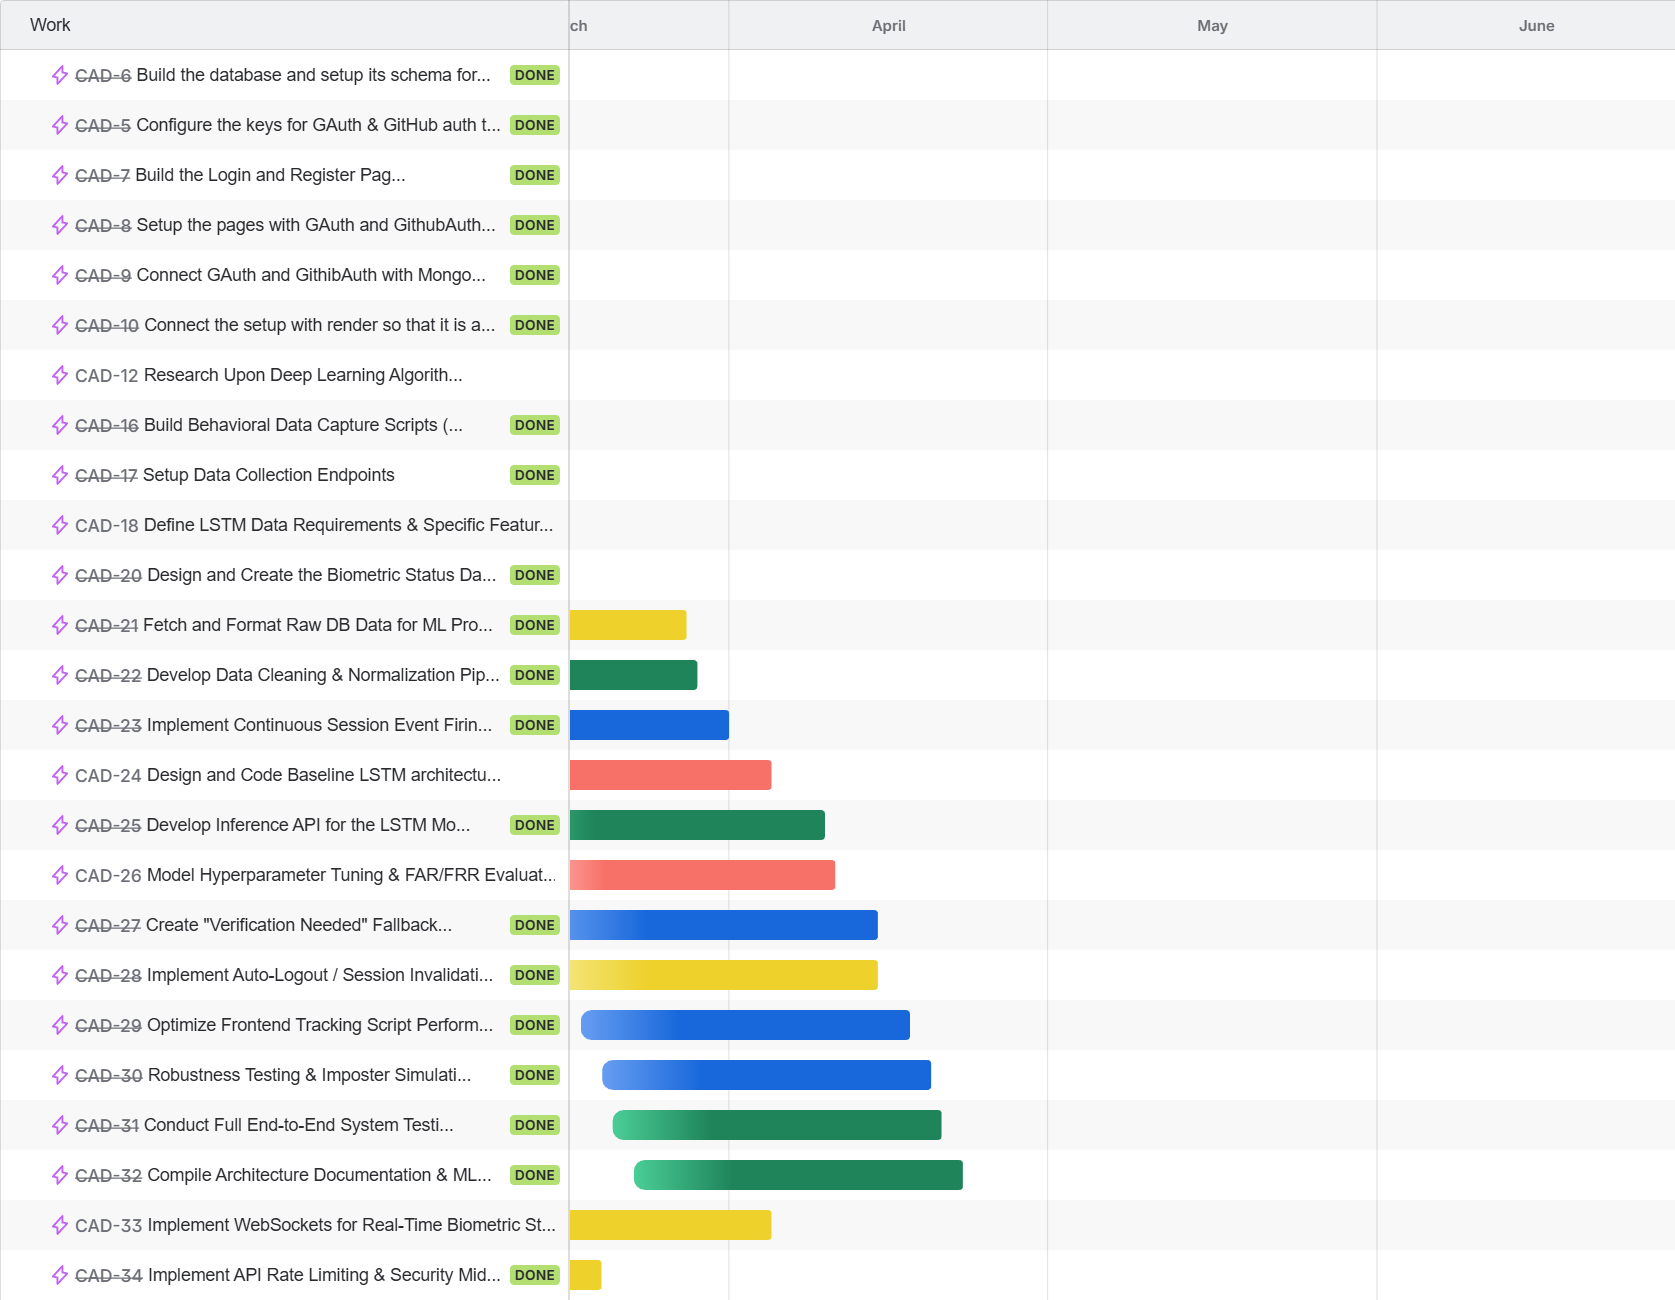
\includegraphics[width=0.9\textwidth]{jira.png} % User MUST upload jira.png
    \caption{Component Granular Task Mapping}
\end{figure}
Task blocks represent specific systemic designs: Models tuning (CAD-26), Real-time sockets (CAD-33), and robust End-to-end testing (CAD-31).

\begin{figure}[H]
    \centering
    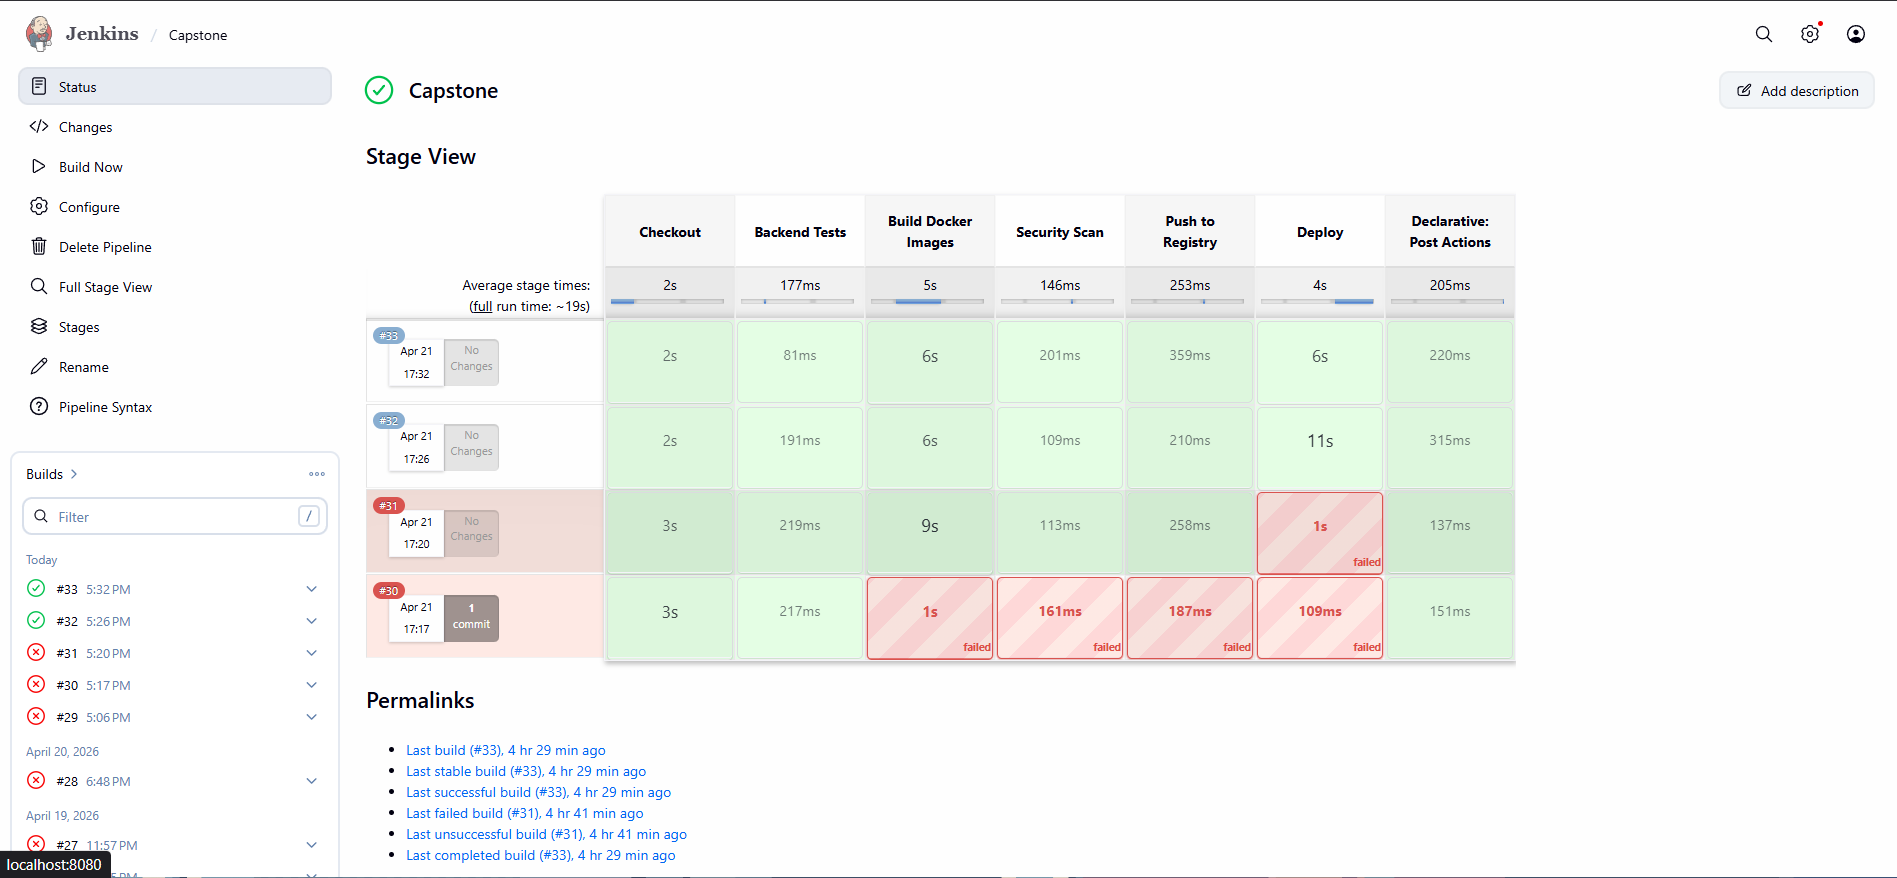
\includegraphics[width=0.9\textwidth]{jenkins.png} % User MUST upload jenkins.png
    \caption{Pipeline CI/CD Historical Durations}
\end{figure}
As analyzed, specific runs illustrate fail-safes actively preventing bad configurations natively. Test durations hover optimally low, verifying architecture responsiveness.

\newpage
\section{Human Interface Design}
\subsection{Overview of User Interface}
The project relies on clean aesthetic boundaries. Standard material buttons and minimal loading screens.

\subsection{Screen Actions}
\begin{itemize}
    \item \textbf{Login Button:} Initiates Google/GitHub flow.
    \item \textbf{Verification Prompts:} Modals appearing upon anomaly triggers. Requires explicit action via camera/microphone authorization.
\end{itemize}

\newpage
\section{Appendices}
\subsection{Technology Stack Index}
\begin{enumerate}
    \item React JS (v18+)
    \item Node.JS / Express Server
    \item MongoDB Atlas
    \item Python 3.10+ (Keras/TensorFlow)
    \item Jenkins Server \& Docker Containerization
\end{enumerate}

\end{document}
